\documentclass[border={8pt 6pt 8pt 6pt}]{standalone}
% Gemeinsamer Preamble fuer die Standalone-Grafiken der Schlusspraesentation.
% Pakete gespiegelt aus src/thesis/hslu_thesis.tex (Z. 56-60), damit die
% extrahierten TikZ-/pgfplots-Grafiken identisch zur Arbeit rendern.
\usepackage[T1]{fontenc}
\usepackage[utf8]{inputenc}
\usepackage{tikz}
\usepackage{pgfplots}
\pgfplotsset{compat=1.18}
\usepgfplotslibrary{groupplots}
\usetikzlibrary{patterns}

\begin{document}
% Extrahiert 1:1 aus chapters/06_validation_und_evaluation.tex (fig:eval_defense_tradeoff).
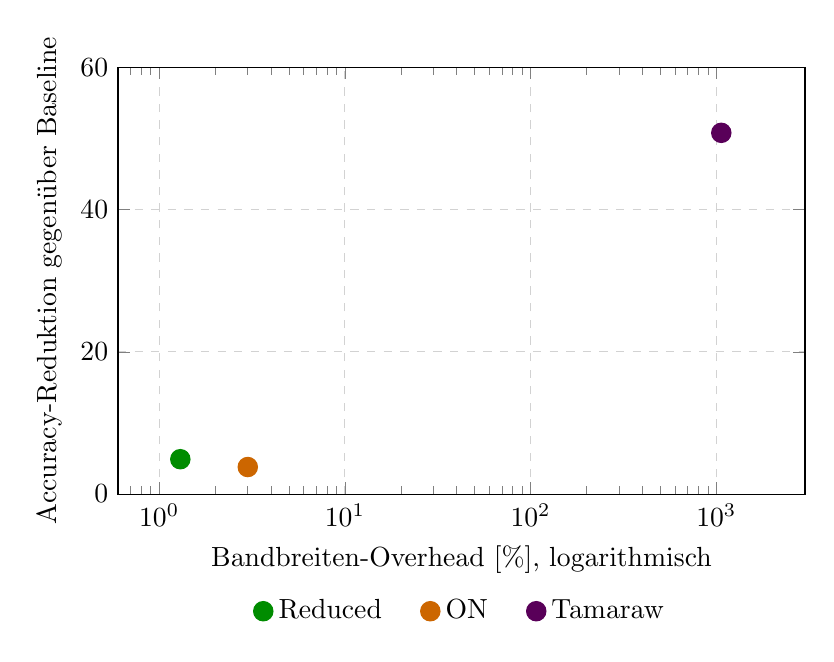
\begin{tikzpicture}
    \begin{semilogxaxis}[
        width=0.85\textwidth,
        height=7cm,
        xlabel={Bandbreiten-Overhead [\%], logarithmisch},
        ylabel={Accuracy-Reduktion gegenüber Baseline},
        xmin=0.6, xmax=3000,
        ymin=0, ymax=60,
        log basis x=10,
        xmajorgrids=true, ymajorgrids=true,
        grid style={dashed, gray!35},
        tick style={black!50},
        legend style={at={(0.5,-0.22)}, anchor=north, legend columns=3, draw=none, /tikz/every even column/.append style={column sep=12pt}},
    ]
        \addplot[only marks, mark=*, mark size=3.5pt, color=green!55!black] coordinates {(1.3, 4.9)};
        \addlegendentry{Reduced}
        \addplot[only marks, mark=*, mark size=3.5pt, color=orange!80!black] coordinates {(3.0, 3.8)};
        \addlegendentry{ON}
        \addplot[only marks, mark=*, mark size=3.5pt, color=violet!70!black] coordinates {(1063.1, 50.8)};
        \addlegendentry{Tamaraw}
    \end{semilogxaxis}
\end{tikzpicture}
\end{document}
